\section{Introduction} 
The goal of this project was not only to automate the processing of the ULTRACAM raw data, but also to provide a mechanism whereby the entire data archive could be made available for easy access to researchers worldwide. The obvious solution is to make the output available through a web enabled interface. From the outset of the project, all efforts have been focused on ensuring that the resulting data is accessible through an easy-to-use web interface. This chapter describes the implementation that was developed for this purpose. 

\section{Web browsers}
In order to enable universal access to the output of the automated pipeline it is important to have a solution that does not require the user to install any additional software on their own computer. We can reasonably safely assume that everyone who has an interest in accessing the ULTRACAM data has a standard web browser installed, a web version of this data archive is the best solution. 

A more specific definition of our assumption is that we expect that the user accessing the archive will have a browser that has the capability of rendering HTML5 markup, Javascript and CSS. These technologies are standard in all popular web browsers in mid-2014. The only notable exception is that Internet Explorer, by Microsoft, is not supported in this project. Although Internet Explorer is a modern browser and does have support for the required technologies, its implementation of these technologies is significantly different to all of the other browsers and would have required extra coding for support. It was felt that, since the majority of astronomers don't use the Microsoft operating system, this omission was justified.  

\section{Web technologies}
HTML, CSS and JavaScript are three core technologies driving the development of the dynamic, interactive and flexible applications we are becoming accustomed to on the web these days. We chose these three technologies to present the ULTRACAM archive. The result is that the reduced archive is immediately available to anyone with a modern web browser and working on any type of computer (desktop, laptop or tablet). There are some high demands on memory, so it is not recommended that the archive is browsed using a mobile phone. There is no lack of functionality that restricts the use of the ULTRACAM site on such a device, but the memory constraints may mean that some runs will not load.  

HTML provides the underlying structure of a modern webpage. It is a semantic markup language, meaning that its purpose is to inform the browser of the document's structure. Despite the habit of many people who dabble at making web pages, HTML is not meant to be used to alter the presentation of content. CSS (or Cascading Style Sheets) markup is designed to inform the browser on how the presentation of each element on the page should look. For example, CSS can define the fonts or colours for each particular element (or set of elements), like headings, paragraphs, etc. JavaScript provides the technology to enable the interactive portion of the page, allowing the user to trigger actions when a mouse is clicked or a new object is loaded. It can be used to manipulate the structure of the existing page. It also provides the mechanism for mathematical computation. Another way of stating this is to say that HTML provides the semantic structure, CSS the presentation layer and JavaScript the programmatic environment. This structure echoes the classic `Model-View-Controller' approach used in many development paradigms in the field of computer science.

The final stage in the ULTRACAM automated pipeline produces a set of files that are available to a web browser. These files are hosted on a web server that is operated by the University of Warwick CSC department. The pipeline prepares the files and then writes them to the appropriate location in the university's local storage. As soon as the pipeline has finished running, the web pages can be viewed globally. 

\label{sect:clientserver}
Web applications like this, are often refered to as 'client-server' applications, meaning that the application consist of two parts, one running on the client (web browser) and the other running on the server of the institution hosting the application. Obviously, there is a one-to-many relationship between clients and server. There is usually only one server involved, but many clients can connect to that server and interact individually with the application. When writing the web interface for this project we had to make a decision on how much of the functionality we should place on the server versus the client. There were two main competing factors to consider:

\emph{Complexity of the application:} Writing an application that has complex components on both the server-side and the client-side, increases the difficulty of writing and maintaining the application. A more sophisticated web server is required such that it is able to run code locally and is able to access local data sources, such as databases. If the application is structured such that all of the complexity is on the client then the web server only needs to host and serve static files. This makes the management of the server-side component trivial. If, on the other hand, the application splits the code to run on both the client and the server, then we need to write code for both components. The connection between client and server can add some latency (time-lag) to the interactions. This would be noticeable if, say, every time the user clicks on a new object in the field, the browser needs to make a new request to the server to fetch an additional of data to render.  

\emph{Browser memory constraints:} Loading all of the data required to display the results of one of the ULTRACAM runs can be quite demanding on the browser. For some runs there are several hundred objects each with several hundred exposures. This can result in a JSON file for the object data that is \textgreater 300 MByte in size. All of this has to be loaded into the browser's memory. If the user is working on a tablet or an older desktop PC or laptop, this can cause memory issues. Some long runs with extremely high cadences have very few objects but hundreds of thousands of exposures and the sheer number of data points will tax the memory management of the browser. That said, it is true that for the vast majority of the runs, the memory load on the browser, although significant, is not a problem. 

In order to aid rapid development of this project, it was decided to opt for a purely client-side code implementation, leaving the web server to serve only static files. By making this decision the burden of computation and memory load is placed on the web browser. This is working adequately in terms of meeting the needs and scope of the project, but it is clear that, for future iterations of this pipeline, careful consideration should be made for moving to an application model that relies more heavily on the server to manipulate, store and serve data. The client cannot take any more of the load. 

Static JSON (JavaScript Object Notation) \footnote{\url{http://json.org/}} files were chosen as the data storage mechanism. This meant that they could be easily loaded by the JavaScript code running on the browser. JavaScript has several built-in methods to load and parse JSON objects. JSON is a flexible, open format that allows a hierarchical structure to be defined for each object stored. It is also designed to be human-readable, meaning that it is possible to open the JSON files in a text editor and check their contents. The problem with this format is that it is stored as plain text and uncompressed. The text itself defines the structure of each object it contains, leading to some amount of redundancy in the file (eg the repeating of labels, etc). While it is true that JSON is inefficient in many ways, it is a useful format to use thanks to its flexibility and the ease with which the developer can check and debug the data. 

Many client-server applications use a relational database to store their data, using a product such as \emph{MySQL}. Since the decision was taken not write any code to run on the server and to only rely on the web server for static files, this did not seem appropriate. It is a topic that will be re-considered when future implementations of the pipeline are planned. 

\section{The Web site}
The core visible product of the project is a website that allows a user to browse all of the data in the ULTRACAM archive. The key features of this website are:
\begin{figure}[!h]
	\centering
	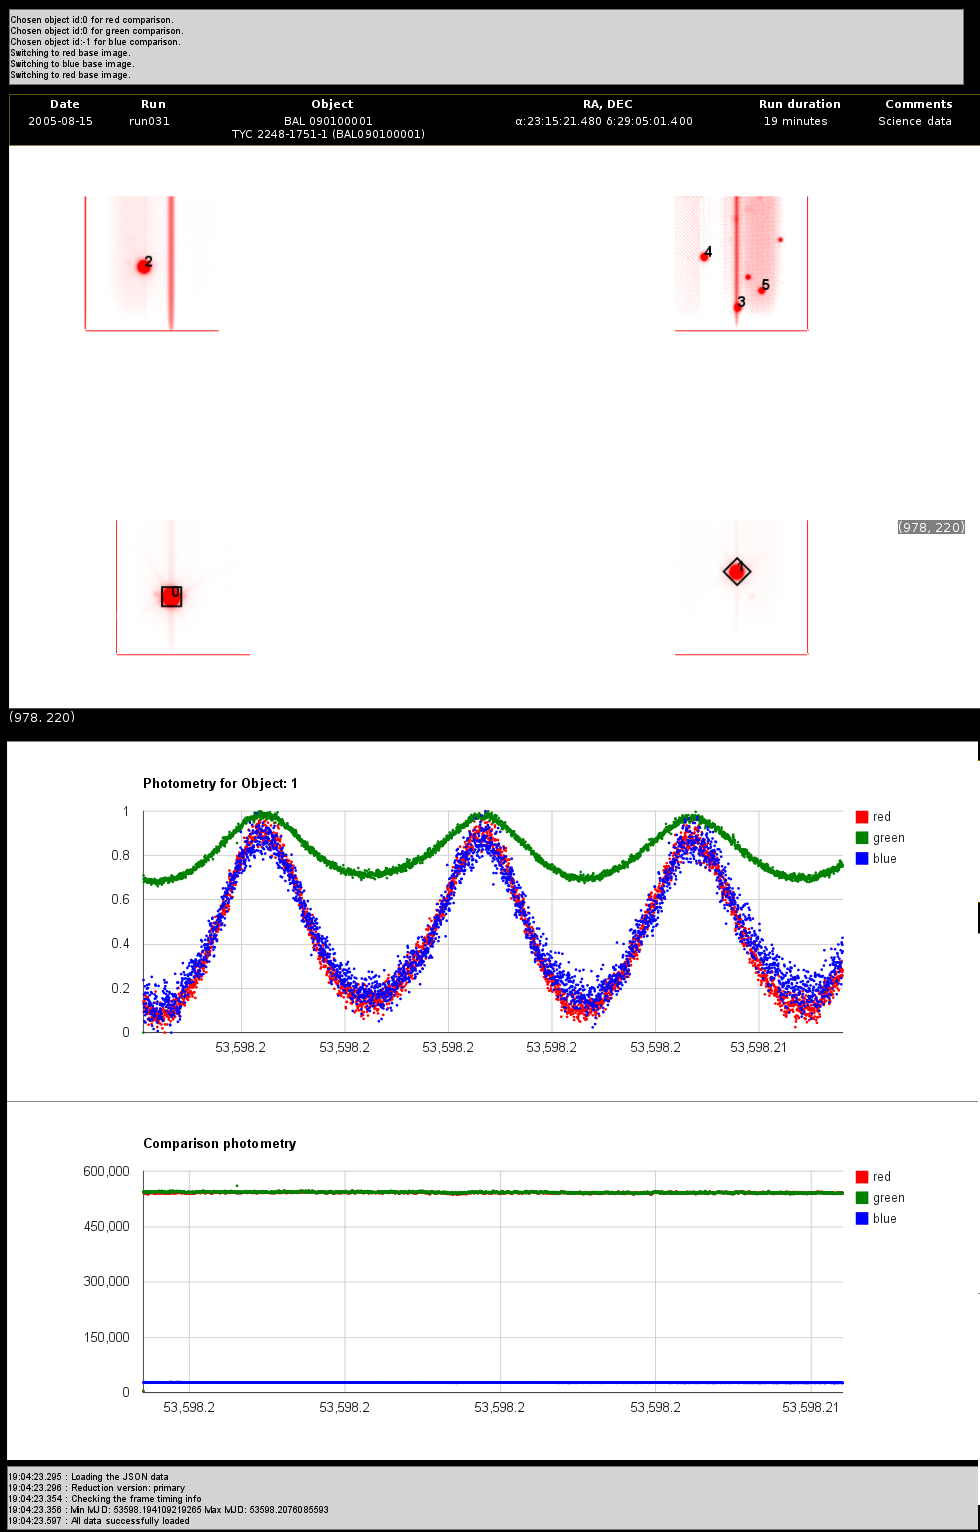
\includegraphics[width=110mm]{images/run031_on_the_night_of_2005-08-15.png}
	\caption{Screen capture of an example web page for browsing the light-curves of a particular run. The object shown is the pulsating sub-dwarf known as TYC 2248-1751-1 or Balloon 090100001.}
	\label{browser}
\end{figure}

\begin{itemize}
	\item A catalog of runs organised by calendar date, containing \emph{thumbnail images} of the fields.
	\item For each run, a web page that shows the user:
	\begin{itemize}
		\item deep images of the field in each of the three channels (r, g, b).
		\item light-curves of each object as the user clicks on the object with the mouse. 
		\item plots of the pixel position of each object over the course of the run.
		\item world coordinates of each object, provided that a correct astrometric solution has been found for the run. 
		\item a light-curve for the object that is currently being used as the 'comparison' object. 
	\end{itemize}
	\item The ability to plot light-curves as absolute measured flux or a relative flux using a selected comparison object in the field. 
	\item The ability to export the data in a CSV format.
	
\end{itemize}
See figure \ref{browser} for an example of the web-page. 


  
\section{Accessing the data}
The pipeline deposits the output HTML, Javascript, image (PNG) and data files (JSON) to a folder that is configured to be served by the University of Warwick's Centre of Scientific Computing (CSC) web server at \url{http://deneb.astro.warwick.ac.uk}. The reader is strongly encouraged to try browsing the archive immediately. It is possible to access the output of any night of observing by entering a URL into the web browser with the following format, \url{http://deneb.astro.warwick.ac.uk/phrnaw/sitedev/YYYY-MM-DD/index.html}. In order to choose a specific night, substitute the \texttt{YYYY-MM-DD} portion of the URL with the appropriate date of the night in question. This will load an HTML page showing all of the runs that occurred during that night. The list will include acquisition runs, biases and flat fields as well as the science runs. The page shows a thumbnail of each run along with a description of the target object, RA and DEC, run duration and the comments entered by the observer at the telescope. Clicking on the run thumbnail leads to the results page for that particular run. Please refer to the user manual in appendix \ref{chap:usermanual} for more details on how to access and browse the data.

\section{Summary}
Once the results of the automated pipeline are placed on the web server, it is  possible to access and browse the light-curves for the ULTRACAM archive. Using the browser it is possible to see reasonably accurate photometry, allowing researchers to make science observations from these data and potentially discover new variable objects. We examine the results of the automated pipeline in the next chapter. 

